\section{clemens\_text}\label{clemens_text} %TODO
 
\subsection{Analyse: BART 2.0}

Analysiert wurde \href{http://www.bart-anaphora.org/}{BART} in der Version 2.0, 
wie sie \href{http://www.bart-anaphora.org/release/bart-2.0.tar.gz}{hier} zu finden 
ist.
Es stehen dem Nutzer zwei Modi zur Nutzung zur Verfügung.
\begin{itemize}
\item BART-WebServer als end-to-end Blackbox Lösung
\item BART-full zum Trainieren eines neuen Modells
\end{itemize}
Erstere erzeugt aus einem Rohtext-Input einen Output, 
wie er in Abb.\ref{bart_webUI_output} zu sehen ist.
Hierfür werden verschiedene Verarbeitungsschritte durchgeführt. 
Diese analysieren jeweils unterschiedliche Ebenen in Syntax und Semantik. 
Beispielhaft hierfür soll der Output der WebServer-Anwendung für die Wortebene in 
Listing\ref{output:bart_word} stehen.

\begin{lstlisting}[label=output:bart_word, name=words.xml, language=xml, caption=BART-Output der Wortebene]
?xml version="1.0" encoding="UTF-8"?>
<!DOCTYPE words SYSTEM "words.dtd">
<words>
  <word id="word_1">Late</word>
  <word id="word_2">in</word>
  <word id="word_3">the</word>
  <word id="word_4">afternoon</word>
  ...
</words>
\end{lstlisting}
Der Output auf Koreferenzebene im XML-Format ist exemplarisch in 
Listing\ref{output:bart_response} dargestellt.
Hierbei ist die Koreferenzkette ,,a low man'' aus Abb.\ref{bart_webUI_output} in dem 
Attribut \lstinline[language=XML]{coref_set="set_4"} kodiert.

\begin{lstlisting}[label=output:bart_response, name=XXX_response_level.xml, language=xml, caption=BART-Output der Koreferenzebene]
<markables>
  ...
  <markable id="markable_51" span="word_120..word_122" coref_set="set_4" min_ids="word_120..word_122" mmax_level="response"/>
  <markable id="markable_13" span="word_128" coref_set="set_4" dir_antecedent="markable_51" mmax_level="response"/>
  <markable id="markable_0" span="word_128..word_129" coref_set="set_0" min_ids="word_128..word_129" mmax_level="response"/>
  ...
</markables>
\end{lstlisting}

\begin{figure}[ht]
\begin{center}
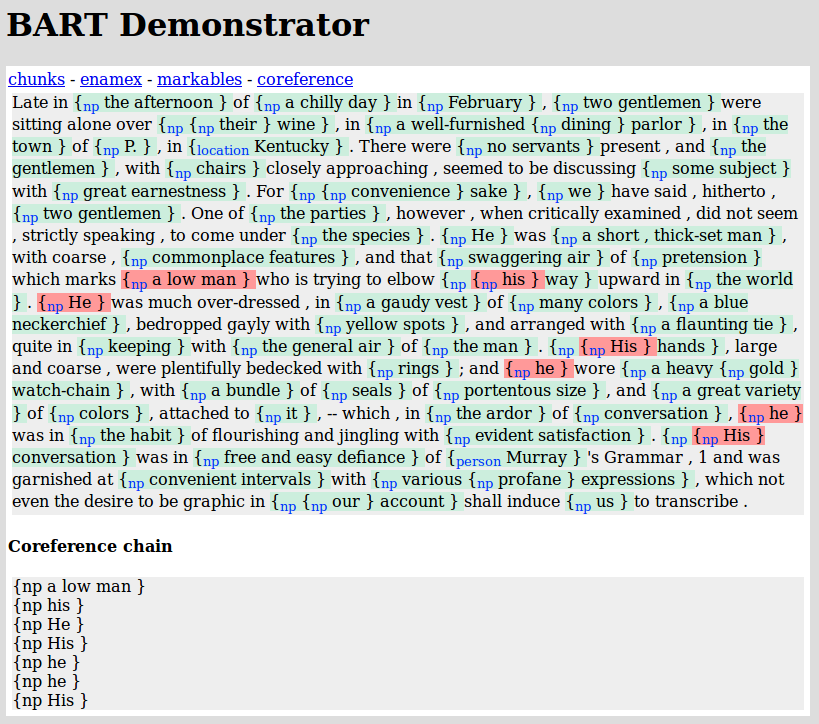
\includegraphics[width=12cm]{./img/cle/bart_webUI_output.png}
 % bart_webUI_output.png: 819x724 pixel, 72dpi, 28.89x25.54 cm, bb=0 0 819 724
\caption{BART 2.0: Output für WebInterface der Blackbox Version}
\label{bart_webUI_output}
\end{center}
\end{figure}

\noindent
Neben der Blackbox-Version bietet BART noch eine Terminalapplikation, 
die zum Trainieren neuer Modelle genutzt werden kann.
Hierfür stehen verschiedene interne Konfigurationsdateien zur Verfügung,
die sich jedoch auf die Weiterverarbeitung beziehen und nicht den erwarteten
Input modifizieren.

Da im Projekt die Verarbeitung von Output des Stanford Parsers gewünscht war,
und wir daher auch innerhalb unserer Gruppe von der Verwendung des MMAX-Formats 
Abstand genommen haben, wurde von der Konvertierung in dieses Format abgesehen.
Eine erste Analyse der Koreferenzketten, die die WebServer-Version von BART ausgab,
unterstützte diese Entscheidung ebenfalls.

 \subsection{Erstellung BuildIndex} %TODO titel